%%%%%%%%%%%%%%%%%%%%%%%%%%%%%%%%%%%%%%%%%
% Professional Mathematical Presentation Template
% 
% This template uses the beamer class with the Madrid theme
% and a custom color scheme for a clean, professional look
% that works well with mathematical content.
%%%%%%%%%%%%%%%%%%%%%%%%%%%%%%%%%%%%%%%%%

\documentclass[aspectratio=169]{beamer} % 16:9 aspect ratio (modern)

% Theme settings
\usetheme{Madrid}
\usecolortheme{default}
\usepackage[dvipsnames]{xcolor}

\definecolor{primcolor}{RGB}{25,50,100} % Dark blue
\setbeamercolor{structure}{fg=primcolor}
\setbeamercolor{frametitle}{bg=primcolor!15, fg=primcolor}
\setbeamercolor{title}{fg=white} % White title text for contrast
\setbeamercolor{subtitle}{fg=white} % White subtitle text
\setbeamercolor{author}{fg=primcolor} % White author text
\setbeamercolor{date}{fg=primcolor} % White date text
\setbeamercolor{institute}{fg=primcolor} % White institute text

% Font settings
\usefonttheme{professionalfonts}
\usefonttheme{serif}

% Package imports
\usepackage{amsmath, amsfonts, amssymb, amsthm} % Math packages
\usepackage{mathtools} % Enhanced math tools
\usepackage{bm} % Bold math symbols
\usepackage{graphicx} % For images
\usepackage{booktabs} % Professional tables
\usepackage{tikz} % For diagrams
\usetikzlibrary{arrows, positioning, matrix, decorations.pathreplacing}

% Use beamer's theorem styles
\setbeamertemplate{theorem}[ams style]
\setbeamertemplate{theorems}[numbered]


% Remove navigation symbols
\setbeamertemplate{navigation symbols}{}

% Custom footer
\setbeamertemplate{footline}{
  \leavevmode%
  \hbox{%
  \begin{beamercolorbox}[wd=.333333\paperwidth,ht=2.25ex,dp=1ex,center]{author in head/foot}%
    \usebeamerfont{author in head/foot}\insertshortauthor
  \end{beamercolorbox}%
  \begin{beamercolorbox}[wd=.333333\paperwidth,ht=2.25ex,dp=1ex,center]{title in head/foot}%
    \usebeamerfont{title in head/foot}\insertshorttitle
  \end{beamercolorbox}%
  \begin{beamercolorbox}[wd=.333333\paperwidth,ht=2.25ex,dp=1ex,right]{date in head/foot}%
    \usebeamerfont{date in head/foot}\insertshortdate{}\hspace*{2em}
    \insertframenumber{} / \inserttotalframenumber\hspace*{2ex} 
  \end{beamercolorbox}}%
  \vskip0pt%
}

% Title information
\title[DP2]{Dynamic Programming}
\subtitle{Thomas J. Sargent and John Stachurski}
\author[Longye]{Longye Tian \\ \texttt{longye.tian@anu.edu.au}}
\institute[ANU]{Australian National University\\ School of Economics}
\date{March 7th, 2025}
\DeclareFontFamily{U}{mathx}{\hyphenchar\font45}
\DeclareFontShape{U}{mathx}{m}{n}{
      <5> <6> <7> <8> <9> <10>
      <10.95> <12> <14.4> <17.28> <20.74> <24.88>
      mathx10
      }{}
\DeclareSymbolFont{mathx}{U}{mathx}{m}{n}
\DeclareMathSymbol{\bigtimes}{1}{mathx}{"91}

\begin{document}

% Title frame
\begin{frame}
  \titlepage
\end{frame}

% Outline frame
\begin{frame}{Outline}
  \tableofcontents
\end{frame}

\begin{frame}{Big Picture}
    
\end{frame}

\begin{frame}{Job Search Model}
    \begin{figure}
        \centering
        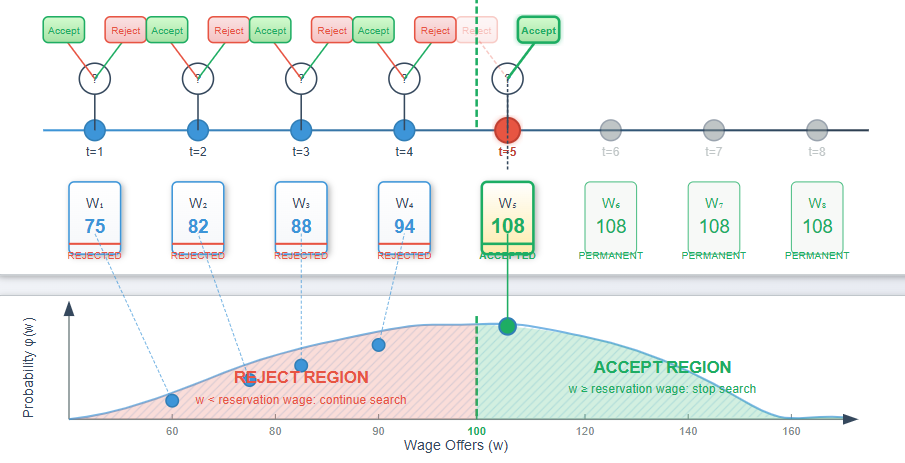
\includegraphics[width=0.95\linewidth]{Dynamic Programming/DP2/Chapter 4/Section 4.1.1. Job Search/Job Search Model.png}
    \end{figure}
\end{frame}


\begin{frame}{Job Search Problem Set up}
    We let 
    \begin{itemize}
        \item $W_t$ denote the wage offer drawn from some fixed distribution $\varphi$
        \item $(W_t)_{t\ge 0}$ is IID and take values from $W\subset \mathbb{R}_+$, \textcolor{blue}{$W$ is nonempty}.
        \item $\varphi$ has finite mean, so $\int w\varphi(dw)<\infty$
        \item Constant discount factor $\beta\in(0,1)$
        \item $L_1(\varphi):= L_1(W,\mathscr{B}, \varphi)$ be all Borel measurable function $f:W\to \mathbb{R}$ with $\int|f|\,d\varphi<\infty$
        \item $\Sigma$ be the set of Borel measurable policy $\sigma: W\to \{0,1\}$
    \end{itemize}
\end{frame}

\begin{frame}{Job Search problem}
We introduce the policy operator $v\mapsto T_\sigma v$ via
$$
(T_\sigma v)(w) = \sigma(w) \frac{w}{1-\beta} + (1-\sigma(w))\left[c+\beta\textcolor{blue}{\underbrace{\int v(w')\, \varphi(dw')}_{\text{Dimension Reduction}}}\right]
$$
    
\end{frame}

\begin{frame}{ADP formulation}
$$
(T_\sigma v)(w) = \sigma(w) \frac{w}{1-\beta} + (1-\sigma(w))\left[c+\beta\textcolor{blue}{\underbrace{\int v(w')\, \varphi(dw')}_{\text{Dimension Reduction}}}\right]
$$

\begin{itemize}
    \item $v\in L^1(\varphi)\implies T_\sigma v\in L^1(\varphi)$
    \item $T_\sigma$ is order preserving self-map on $L^1(\varphi)$
    \item $\Sigma$ is not empty
\end{itemize}
$$
(L^1(\varphi),\mathbb{T}_{JS}), \quad \mathbb{T}_{JS}:=\{T_\sigma: \sigma\in\Sigma\}
$$
is an ADP for the Job Search Problem. 
\end{frame}

\begin{frame}{The ADP $(L^1(\varphi),\mathbb{T}_{JS})$ is well-posed.}
 $$
 (T_\sigma v)(w) = v(w) 
 $$
 $$
\implies
 $$
    $$
\sigma(w) \frac{w}{1-\beta} + (1-\sigma(w))\left[c+\beta\int v(w')\, \varphi(dw')\right] = v(w)
$$

\begin{itemize}
    \item $\sigma(w) = 1 \implies v(w) = \frac{w}{1-\beta} $ well-defined and unique
    \item $\sigma(w) = 0\implies v(w) = c+\beta\int v(w') \, \varphi(dw')$ well-defined and unique
\end{itemize}

\end{frame}

\begin{frame}{The ADP $(L^1(\varphi),\mathbb{T}_{JS})$ is regular}
$v$-greedy policy (assume accept the offer at indifference)
    $$
    \sigma (w) = \mathbf{1}\left\{\frac{w}{1-\beta}\ge c+\beta\int v(w') \, \varphi(dw') \right\}
    $$
    with policy operator
    $$
    (T_\sigma v)(w) = \max\left\{\frac{w}{1-\beta}, c+\beta\int v(w') \, \varphi(dw')\right\} \textcolor{blue}{\underbrace{= (Tv)(w)}_{\text{greedy}}}
    $$
\end{frame}

\begin{frame}{Construct Bellman operator from definition}
    $Tv = \bigvee_\sigma T_\sigma v$
    \begin{align*}
        (Tv)(w) &= \left(\bigvee_\sigma T_\sigma v\right)(w)\\
        &= \bigvee_\sigma \left(\sigma(w) \frac{w}{1-\beta} + (1-\sigma(w))\left[c+\beta\int v(w')\, \varphi(dw')\right]\right)\\
        &= \max\left\{\frac{w}{1-\beta}, c+\beta\int v(w') \, \varphi(dw')\right\}
    \end{align*}
    
\end{frame}

\begin{frame}{Bounded $W$ $\implies$ use smaller value space}
$$
\sigma(w) \frac{w}{1-\beta} + (1-\sigma(w))\left[c+\beta\int v(w')\, \varphi(dw')\right]
$$
\begin{itemize}
    \item From $L^1(\varphi)$ to \textcolor{blue}{$bmW$} bounded Borel measurable function
    \item From \textcolor{blue}{$bmW$} to \textcolor{ForestGreen}{$bcW$} bounded continuous function
    \item From \textcolor{ForestGreen}{$bcW$} to \textcolor{Lavender}{$ibcW$} increasing bounded continuous function
    \item From \textcolor{Lavender}{$ibcW$} to \textcolor{RedOrange}{$ibcW_+$} nonnegative increasing bounded continuous function
\end{itemize}
\end{frame}

\begin{frame}{Job Search is RDP}
    
\end{frame}


\begin{frame}{Optimality with IID offers}
    \begin{proposition}
        For $(L^1(\varphi),\mathbb{T}_{JS})$,
        \begin{itemize}
            \item the fundamental optimality properties hold
            \item VFI, OPI, HPI all converge.
        \end{itemize}
    \end{proposition}
\end{frame}

\end{document}
